\subsection*{Set Operations and Functions Acting on Sets}
We will now consider the following situation:  Let $S$ and $T$ be sets and let $f$ be a function from $S$ to $T$.  Also, let $A$ and $B$ be subsets of $S$ and let $C$ and $D$ be subsets of $T$.  In the remainder of this section, we will consider the following situations and answer the questions posed in each case.

\begin{itemize}
\item The set $A \cap B$ is a subset of $S$ and so $f ( A \cap B )$ is a subset of $T$.  In addition, $f ( A )$ and $f ( B )$ are subsets of $T$.  Hence, 
$f ( A ) \cap f ( B )$ is a subset of $T$.

\noindent
Is there any relationship between $f ( A \cap B )$ and 
$f ( A ) \cap f ( B )$?


\item The set $A \cup B$ is a subset of $S$ and so $f ( A \cup B )$ is a subset of $T$.  In addition, $f ( A )$ and $f ( B )$ are subsets of $T$.  Hence, 
$f ( A ) \cup f ( B )$ is a subset of $T$.

\noindent
Is there any relationship between $f ( A \cup B )$ and 
$f ( A ) \cup f ( B )$?

\item The set $C \cap D$ is a subset of $T$ and so $f^{-1} ( C \cap D )$ is a subset of $S$.  In addition, $f^{-1} ( C )$ and $f^{-1} ( D )$ are subsets of $S$. Hence, $f^{-1} ( C ) \cap f^{-1} ( D )$ is a subset of $S$.

\noindent
Is there any relationship between the sets $f^{-1} ( C \cap D )$ and \linebreak 
$f^{-1} ( C ) \cap f^{-1} ( D )$?

\item The set $C \cup D$ is a subset of $T$ and so $f^{-1} ( C \cup D )$ is a subset of $S$.  In addition, $f^{-1} ( C )$ and $f^{-1} ( D )$ are subsets of $S$. Hence, $f^{-1} ( C ) \cup f^{-1} ( D )$ is a subset of $S$.

\noindent
Is there any relationship between the sets $f^{-1} ( C \cup D )$ and \linebreak
$f^{-1} ( C ) \cup f^{-1} ( D )$?
\end{itemize}

\noindent
These and other questions will be explored in the next progress check.
\hbreak

\begin{prog}[\textbf{Set Operations and Functions Acting on Sets}] \label{prog:setsandfunctions} \hfill \\
In Section~\ref{S:moreaboutfunctions}, we introduced functions involving congruences.  For example, if we let
\[
R_8 = \left\{0, 1, 2, 3, 4, 5, 6, 7 \right\},
\]
then we can define $f\x  R_8 \to R_8$ by $f ( x ) = r$, where 
$\left( x^2 + 2 \right) \equiv r \pmod 8$ and $r \in R_8$.  Moreover, we shortened this notation to
\[
f ( x ) = \left( x^2 + 2 \right) \pmod 8 .
\]
%\noindent
%\textbf{Special Note for Those Who Have Studied Section~\ref{S:modulararithmetic}} \hfill
%
%In Section~\ref{S:modulararithmetic}, we used the notation $R_8$ to represent the set of all congruence classes of the integers for the equivalence relation of congruence modulo 8.  That is,
%\[
%R_8 = \left\{\left[ 0 \right], \left[ 1 \right], \left[ 2 \right], \left[ 3 \right], 
%\left[ 4 \right], \left[ 5 \right], \left[ 6 \right], \left[ 7 \right] \right\}.
%\]
%In this notation, we are in effect using one integer inside brackets to represent an entire congruence class.  So to make the notation somewhat easier to use, we are dropping the brackets and just writing the integer to represent the congruence class.
%\vskip6pt


\noindent
We will use the following subsets of $\R_8$:
$$
\BeginTable
\BeginFormat
| c | c | c | c |
\EndFormat
" $A = \left\{ 1, 2, 4 \right\}$ " $B = \left\{ 3, 4, 6 \right\}$ " 
$C = \left\{ 1, 2, 3 \right\}$ " $D = \left\{ 3, 4, 5 \right\}$. " \\
\EndTable
$$


\begin{enumerate}
\item Verify that $f ( 0 ) = 2$, $f ( 1 ) = 3$, $f ( 2 ) = 6$, and $f ( 3 ) = 3$.  Then determine $f ( 4 )$, $f ( 5 )$, 
$f ( 6 )$, and $f ( 7 )$.
\item Determine $f (A )$, $f (B )$, $f^{-1} (C )$, and 
$f^{-1} (D )$.


\item For each of the following, determine the two subsets of $R_8$ and then determine if there is a relationship between the two sets.  For example,  
$A \cap B = \left\{ 4 \right\}$ and since $f(4) = 2$, we see that 
$f ( A \cap B ) = \left\{ 2 \right\}$.
\begin{enumerate}
\item $f ( A \cap B )$ and $f ( A ) \cap f ( B )$
\item $f ( A \cup B )$ and $f ( A ) \cup f ( B )$
\item $f^{-1} ( C \cap D )$ and $f^{-1} ( C ) \cap f^{-1} ( D )$
\item $f^{-1} ( C \cup D )$ and $f^{-1} ( C ) \cup f^{-1} ( D )$
\end{enumerate}

\item Notice that $f ( A )$ is a subset of the codomain, $R_8$.  Consequently, 
\linebreak
$f^{-1} \!\left( f ( A ) \right)$ is a subset of the domain, 
$R_8$.  Is there any relation between $A$ and $f^{-1} \!\left( f ( A ) \right)$ in this case?

\item Notice that $f^{-1} ( C )$ is a subset of the domain, $R_8$.  Consequently, 
\linebreak
$f \!\left( f^{-1} ( C ) \right)$ is a subset of the codomain, 
$R_8$.  Is there any relation between $C$ and $f \!\left( f^{-1} ( C ) \right)$ in this case?
\end{enumerate}
\end{prog}
\hbreak

\begin{example}[\textbf{Set Operations and Functions Acting on Sets}] \label{exam:setsandfunctions2} \hfill \\
Define $f\x  \mathbb{R} \to \mathbb{R}$ by $f ( x ) = x^2 + 2$ for all 
$x \in \mathbb{R}$.  It will be helpful to use the graph shown in Figure~\ref{fig:examplein91}.
\begin{figure}[h]
\begin{center}

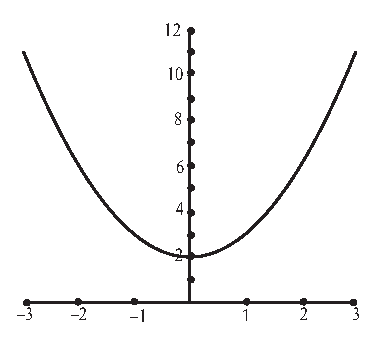
\includegraphics{figps-setsandfunctions.eps} 
\caption{Graph for Example~\ref{exam:setsandfunctions2}} \label{fig:examplein91}
\end{center}
\end{figure}

\noindent
We will use the following closed intervals:
$$
\BeginTable
\BeginFormat
| c | c | c | c |
\EndFormat
" $A = \left[ 0, 3 \right]$ " $B = \left[ -2, 1\right]$ 
" $C = \left[ 2, 6 \right]$ " $D = \left[ 0, 3 \right]$. " \\
\EndTable
$$
\begin{enumerate}
\item Verify that $f ( A ) = [2, 11]$, $f ( B ) = [2, 6]$, 
$f^{-1} ( C ) = [-2, 2]$, and that $f^{-1} ( D ) = [-1, 1]$.

\item \begin{enumerate}
\item Explain why $f ( A \cap B ) = [2, 3]$ and 
$f ( A ) \cap f ( B ) = [2, 6]$.  So in this case, 
$f ( A \cap B ) \subseteq f ( A ) \cap f ( B )$.

\item Explain why $f ( A \cup B ) = [2, 11]$ and 
$f ( A ) \cup f ( B ) = [2, 11]$.  So in this case, 
$f ( A \cup B ) = f ( A ) \cup f ( B )$.

\item Explain why $f^{-1} ( C \cap D ) = [-1, 1]$ and 
$f^{-1} ( C ) \cap f^{-1} ( D ) = [-1, 1]$.  So in this case,
$f^{-1} ( C \cap D ) = f^{-1} ( C ) \cap f^{-1} ( D )$.

\item Explain why $f^{-1} ( C \cup D ) = [-2, 2]$ and 
$f^{-1} ( C ) \cup f^{-1} ( D ) = [-2, 2]$.  So in this case, 
$f^{-1} ( C \cup D ) = f^{-1} ( C ) \cup f^{-1} ( D )$.
\end{enumerate}

\item Recall that $A = [0, 3]$.  Notice $f ( A ) = [2, 11]$ is a subset of the codomain, $\mathbb{R}$. Explain why $f^{-1} \!\left( f ( A ) \right) = [-3, 3]$.  Since  
$f^{-1} \!\left( f ( A ) \right)$ is a subset of the domain, 
$\mathbb{R}$, we see that in this case, 
$A \subseteq f^{-1} \!\left( f ( A ) \right)$.

\item Recall that $C = [2, 6]$.  Notice that $f^{-1} ( C ) = [-2, 2]$ is a subset of the domain, 
$\mathbb{R}$.  Explain why $f \!\left( f^{-1} ( C ) \right) = [2, 6]$.  Since 
$f \!\left( f^{-1} ( C ) \right)$ is a subset of the codomain, 
$\mathbb{R}$, we see that in this case $f \!\left( f^{-1} ( C ) \right) = C$.
\end{enumerate}
\end{example}
\hbreak

The examples in Progress Check~\ref{prog:setsandfunctions} and 
Example~\ref{exam:setsandfunctions2} were meant to illustrate general results about how functions act on sets.  In particular, we investigated how the action of a function on sets interacts with the set operations of intersection and union.  We will now state the theorems that these examples were meant to illustrate.  Some of the proofs will be left as exercises.

\begin{theorem} \label{T:imageofoperations}
Let $f\x S \to T$ be a function and let $A$ and $B$ be subsets of $S$.  Then
\begin{enumerate}
\item $f ( A \cap B ) \subseteq f ( A ) \cap f ( B )$
\label{T:imageofoperations1}
\index{image!of an intersection}%

\item $f ( A \cup B ) = f ( A ) \cup f ( B )$
\label{T:imageofoperations2}
\index{image!of a union}%
\end{enumerate}
\end{theorem}
%
\begin{myproof}
We will prove Part~(\ref{T:imageofoperations1}).  The proof of 
Part~(\ref{T:imageofoperations2}) is Exercise~(\ref{exer:sec91-5}).

Assume that $f\x S \to T$ is a function and let $A$ and $B$ be subsets of $S$.  We will prove that $f ( A \cap B ) \subseteq f ( A ) \cap f ( B )$ by proving that for all $y \in T$, if $y \in f ( A \cap B )$, then 
$y \in f ( A ) \cap f ( B )$.

We assume that $y \in f ( A \cap B )$.  This means that there exists an 
$x \in A \cap B$ such that $f ( x ) = y$.  Since $x \in A \cap B$, we conclude that 
$x \in A$ and $x \in B$.

\begin{itemize}
\item Since $x \in A$ and $f ( x ) = y$, we conclude that $y \in f ( A )$.

\item Since $x \in B$ and $f ( x ) = y$, we conclude that $y \in f ( B )$.
\end{itemize}
Since $y \in f ( A )$ and $y \in f ( B )$,  
$y \in f ( A ) \cap f ( B )$.  This proves that if 
$y \in f ( A \cap B )$, then $y \in f ( A ) \cap f ( B )$.  Hence $f ( A \cap B ) \subseteq f ( A ) \cap f ( B )$.
\end{myproof}
%\hrule
%
\eighth

\begin{theorem} \label{T:invimageofoperations}
Let $f\x S \to T$ be a function and let $C$ and $D$ be subsets of $T$.  Then
\begin{enumerate}
\item $f^{-1} ( C \cap D ) = f^{-1} ( C ) \cap f^{-1} ( D )$
\label{T:invimageofoperations1}
\index{preimage!of an intersection}%

\item $f^{-1} ( C \cup D ) = f^{-1} ( C ) \cup f^{-1} ( D )$
\label{T:invimageofoperations2}
\index{preimage!of a union}%
\end{enumerate}
\end{theorem}
%
\begin{myproof}
We will prove Part~(\ref{T:invimageofoperations2}).  The proof of 
Part~(\ref{T:invimageofoperations1}) is Exercise~(\ref{exer:sec91-6}).

Assume that $f\x S \to T$ is a function and that $C$ and $D$ are subsets of $T$.  We will prove that $f^{-1} ( C \cup D ) = f^{-1} ( C ) \cup f^{-1} ( D )$ by proving that each set is a subset of the other.

We start by letting $x$ be an element of $f^{-1} ( C \cup D )$.  This means that 
$f ( x )$ is an element of $C \cup D$.  Hence,
\[
f ( x ) \in C \text{ or } f ( x ) \in D.
\]
In the case where $f ( x ) \in C$, we conclude that $x \in f^{-1} ( C )$, and hence that $x \in f^{-1} ( C ) \cup f^{-1} ( D )$.  In the case where $f ( x ) \in D$, we see that $x \in f^{-1} ( D )$, and hence that 
$x \in f^{-1} ( C ) \cup f^{-1} ( D )$.  So in both cases, 
$x \in f^{-1} ( C ) \cup f^{-1} ( D )$, and we have proved that 
$f^{-1} ( C \cup D ) \subseteq f^{-1} ( C ) \cup f^{-1} ( D )$.

We now let $t \in f^{-1} ( C ) \cup f^{-1} ( D )$.  This means that
\[
t \in f^{-1} ( C ) \text{ or } t \in f^{-1} ( D ).
\]
\begin{itemize}
\item In the case where $t \in f^{-1} ( C )$, we conclude that 
$f ( t ) \in C$ and hence that $f ( t ) \in C \cup D$.  This means that 
$t \in f^{-1} ( C \cup D )$.

\item Similarly, when $t \in f^{-1} ( D )$, it follows that 
$f ( t ) \in D$ and hence that $f ( t ) \in C \cup D$.  This means that 
$t \in f^{-1} ( C \cup D )$.
\end{itemize}

These two cases prove that if $t \in f^{-1} ( C ) \cup f^{-1} ( D )$, then 
$t \in f^{-1} ( C \cup D )$.  Therefore, 
$f^{-1} ( C ) \cup f^{-1} ( D ) \subseteq f^{-1} ( C \cup D )$.

Since we have now proved that each of the two sets is a subset of the other set, we can conclude that $f^{-1} ( C \cup D ) = f^{-1} ( C ) \cup f^{-1} ( D )$.
\end{myproof}
%\hrule
%
%\pagebreak
\begin{theorem} \label{T:imageofinvimage}
Let $f\x S \to T$ be a function and let $A$ be a subset of $S$ and let $C$ be a subset of $T$.  Then
\begin{multicols}{2}
\begin{enumerate}
\item $A \subseteq f^{-1} \!\left( f ( A ) \right)$
\label{T:imageofinvimage1}

\item $f \!\left( f^{-1} ( C ) \right) \subseteq C$
\label{T:imageofinvimage2}
\end{enumerate}
\end{multicols}
\end{theorem}
%
\begin{myproof}
We will prove Part~(\ref{T:imageofinvimage1}).  The proof of 
Part~(\ref{T:imageofinvimage2}) is Exercise~(\ref{exer:sec91-7}).

To prove Part~(\ref{T:imageofinvimage1}), we will prove that for all $a \in S$, if $a \in A$, then \linebreak 
$a \in f^{-1} \!\left( f ( A ) \right)$.  So let $a \in A$.  Then, by definition, 
$f ( a ) \in f ( A )$.  We know that $f ( A ) \subseteq T$, and so 
$f^{-1} \!\left( f ( A ) \right) \subseteq S$.  Notice that
\[
f^{-1} \!\left( f ( A ) \right) = \left\{ x \in S \mid f ( x ) \in 
f ( A ) \right\}.
\]
Since $f ( a ) \in f ( A )$, we use this to conclude that 
$a \in f^{-1}\!\left ( f ( A ) \right)$.  This proves that if $a \in A$, then 
$a \in f^{-1} \!\left( f ( A ) \right)$, and hence that 
$A \subseteq f^{-1} \!\left( f ( A ) \right)$.
\end{myproof}
\hbreak

\endinput
